% %%%%%%%%%%%%%%%%%%%%%%%%%%%%%%%%%%%%%%%%%%%%%%%%%%%%%%%%%%%%%%%%%%%%%%%%%%%%%%%%%%
% \begin{frame}[fragile]\frametitle{}
% \begin{center}
% {\Large Notes from Teachings of Krishna Prakash of Shrimath}
% \end{center}
% \end{frame}

% %%%%%%%%%%%%%%%%%%%%%%%%%%%%%%%%%%%%%%%%%%%%%%%%%%%%%%%%%%%
% \begin{frame}[fragile]\frametitle{Starting Yoga}

	% \begin{itemize}
	% \item Yoga Sadhna is An Endless Ocean	
	% \item You cannot be a Yoga Teacher/Guru just after training or certification, practice it for years (12), experience the benefits, then only teach.
	% \item Small Sized Yoga Classes is a Must
	% \item Meditation instructions lack emphasis on posture.
	% \item Still Your Body and Steady Mind
	% \item Persist with spiritual practices Long Enough
	% \item Guru emphasizes endless hours, and dedication for yoga.
	% \item Without steadiness, meditation cannot happen e.g. curd sets when still
	% \item Asana brings steadiness and Pranayama brings lightness, pratyahara brings witness-bhava
	% \item Pavanmuktasana series by Satyananda, of 34 Asanas To Start Yoga Journey
	% \end{itemize}

% {\tiny (Ref:  I Did yoga for 7 Days Following A Yogi's Advice- With ‪@ShrimathYoga‬  spirituality - Tathastu - Secrets of Bharat)}

% \end{frame}

% %%%%%%%%%%%%%%%%%%%%%%%%%%%%%%%%%%%%%%%%%%%%%%%%%%%%%%%%%%%
% \begin{frame}[fragile]\frametitle{Immunity}

% \begin{columns}
    % \begin{column}[T]{0.6\linewidth}
		% \begin{itemize}
		% \item 340 important pressure points on the body with which health can be managed. 28 are on palms. Clapping for upto 20 minutes before meals
		% \item 'PraN Mudra' (thumb and last two small fingers touching) 12 minutes
		% \item 'Ling Mudra' (fist clasped, left thumb upward, keep at naval) 12 minutes
		% \item Bhramari Pranayam + Khechari Mudra, inhale without sound, exhale with bee sound from tight throat. 7 minutes, 3 times a day.
		% \end{itemize}

    % \end{column}
    % \begin{column}[T]{0.4\linewidth}
		% \begin{center}
		% 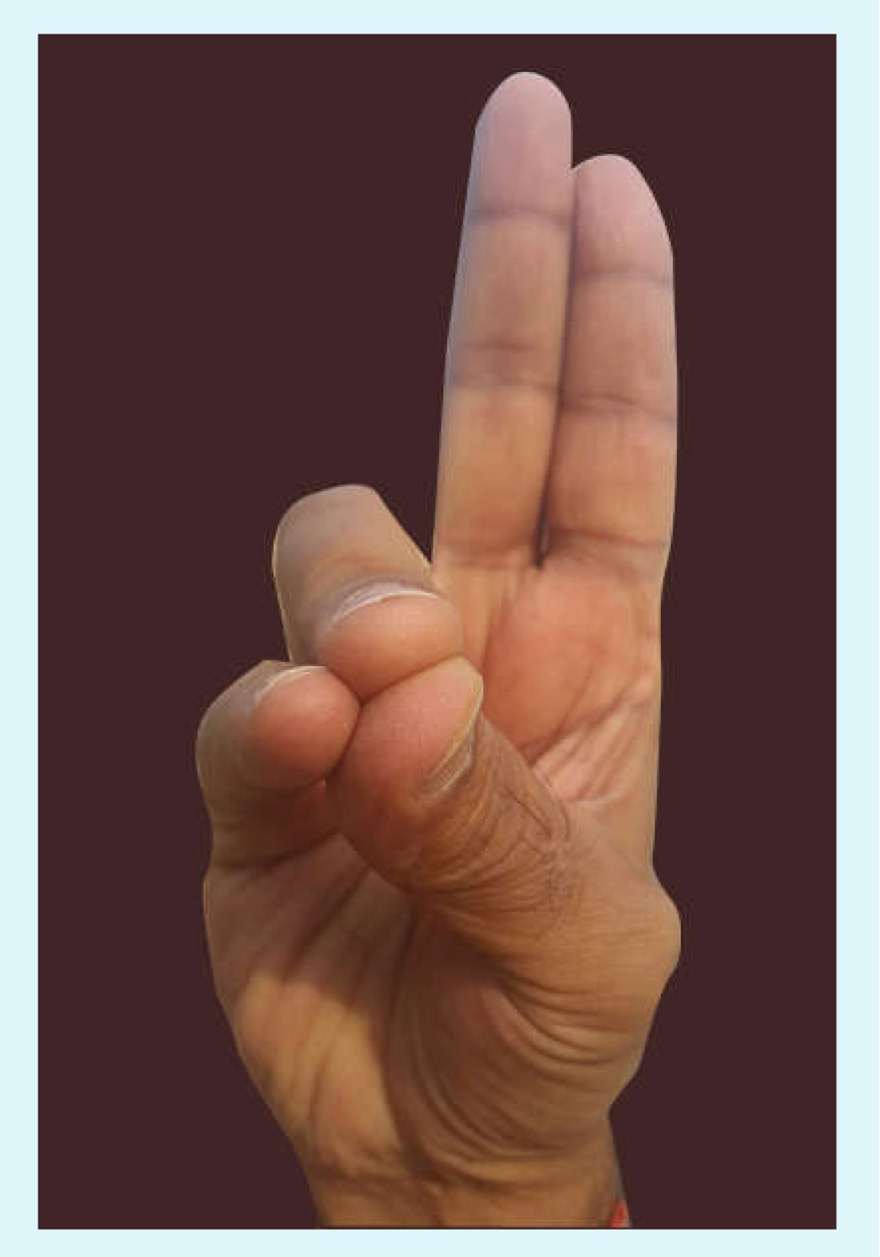
\includegraphics[width=0.4\linewidth,keepaspectratio]{pranmudra}
		
		% 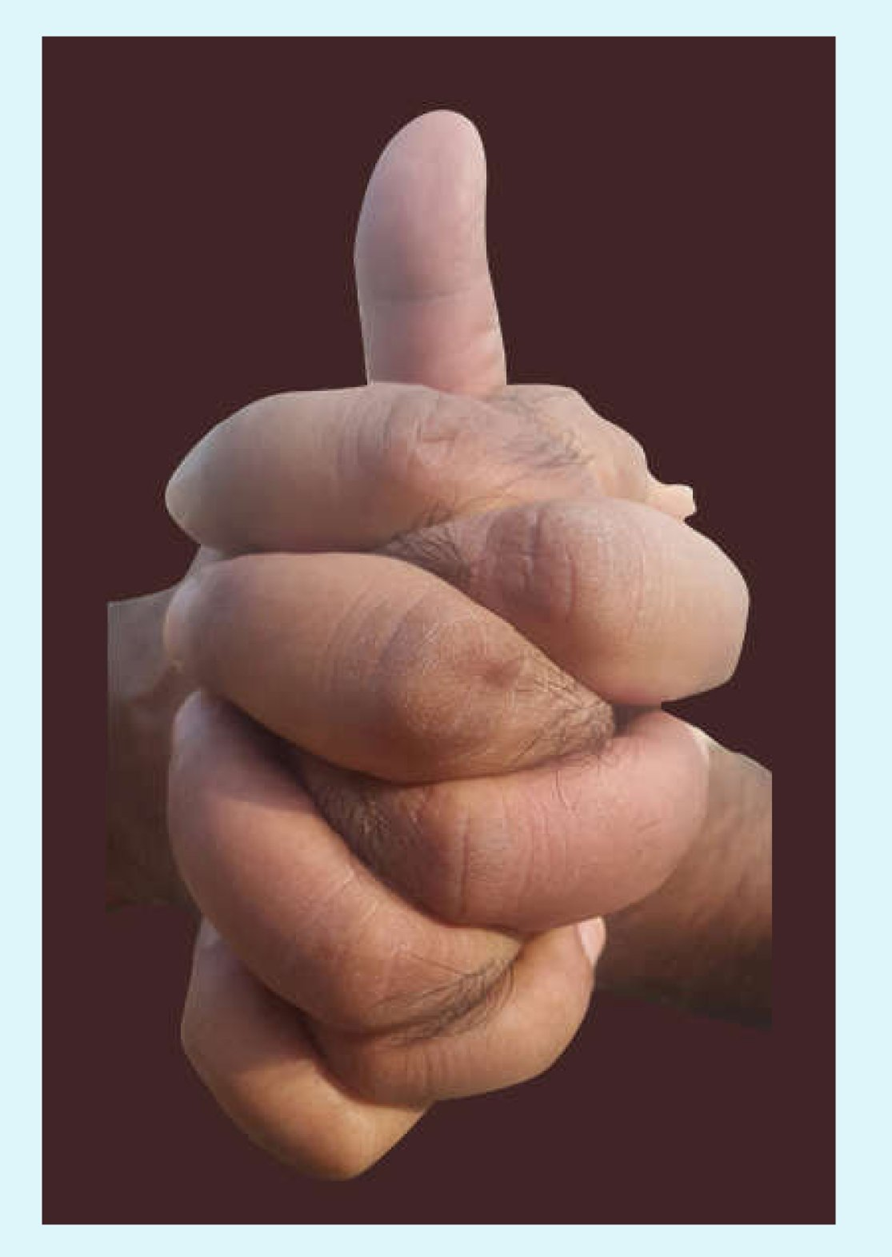
\includegraphics[width=0.4\linewidth,keepaspectratio]{lingmudra}
		
		% \end{center}	
    % \end{column}
  % \end{columns}
  


% {\tiny (Ref:  Building Immunity 2.0 - Shrimath Yoga)}

% \end{frame}

%%%%%%%%%%%%%%%%%%%%%%%%%%%%%%%%%%%%%%%%%%%%%%%%%%%%%%%%%%%%%%%%%%%%%%%%%%%%%%%%%%
\begin{frame}[fragile]\frametitle{}
\begin{center}
{\Large Inner Silence}
\end{center}

{\tiny (Ref:  Master Class on Antar Mouna Level 1 - Shrimath Yoga)}

\end{frame}

%%%%%%%%%%%%%%%%%%%%%%%%%%%%%%%%%%%%%%%%%%%%%%%%%%%%%%%%%%%
\begin{frame}[fragile]\frametitle{What is Inner Silence?}
    \begin{itemize}
        \item Practice of Pratyahara प्रत्याहार : Withdrawing is difficult as our nature is to seek knowledge.
        \item Vedanta: Our Ultimate Reality is Sat Chid Anand. सत् चित् आनन्द 
        \item \textbf{Sat सत्} - Pure existence, why we wish to live forever.
        \item \textbf{Chit चित् } - Consciousness, reason for our thirst for knowledge.
        \item \textbf{Ananda} - Pure bliss, reason we avoid sadness.
    \end{itemize}
\end{frame}

%%%%%%%%%%%%%%%%%%%%%%%%%%%%%%%%%%%%%%%%%%%%%%%%%%%%%%%%%%%
\begin{frame}[fragile]\frametitle{Understanding Sat सत्  Chit चित्  Anand आनन्द}
    \begin{itemize}
        \item We fear death because of our attachment to existence (Sat सत्).
        \item Knowledge is innate; absence of it makes us restless (Chit चित् ).
        \item We resist sadness as our nature is bliss (Ananda आनन्द).
        \item Stress, annoyance, and irritation arise from deviation from bliss.
    \end{itemize}
\end{frame}

%%%%%%%%%%%%%%%%%%%%%%%%%%%%%%%%%%%%%%%%%%%%%%%%%%%%%%%%%%%
\begin{frame}[fragile]\frametitle{Ocean Analogy \& Realization}
    \begin{itemize}
        \item Waves exist only near the shore; deep ocean remains still.
        \item Inner silence grows with experience and realization.
        \item Excess money, fame, or power do not equate to true calmness.
        \item True peace comes from within, not from external achievements.
    \end{itemize}
\end{frame}

%%%%%%%%%%%%%%%%%%%%%%%%%%%%%%%%%%%%%%%%%%%%%%%%%%%%%%%%%%%
\begin{frame}[fragile]\frametitle{Withdrawal - The Key to Inner Silence}
    \begin{itemize}
        \item Managing the five senses is the first level of inner silence.
        \item Sensory pulls appear enticing but cause distractions.
        \item Regular withdrawal helps recuperate and maintain balance.
        \item Use senses to transcend distractions, not be controlled by them.
    \end{itemize}
\end{frame}

%%%%%%%%%%%%%%%%%%%%%%%%%%%%%%%%%%%%%%%%%%%%%%%%%%%%%%%%%%%
\begin{frame}[fragile]\frametitle{Antar Mouna अंतर मौन  - The Battle Within}
    \begin{itemize}
        \item Practiced amidst daily life, not in isolation.
        \item 6 levels of Antar Mouna:
        \item \textbf{Level 1}: Live with sensory pulls, accept distractions.
        \item Do not give control of your mind to external factors.
        \item Listing and observing distractions helps detach from them.
        \item Avoidance increases suffering; face challenges and evolve.
    \end{itemize}
\end{frame}

%%%%%%%%%%%%%%%%%%%%%%%%%%%%%%%%%%%%%%%%%%%%%%%%%%%%%%%%%%%
\begin{frame}[fragile]\frametitle{Developing Inner Silence}
    \begin{itemize}
        \item Swami Satyananda स्वामी सत्यानंद : Inner silence $=$ mind aware of external sounds.
        \item Awareness of sounds brings moments of quietness within.
        \item Gradually, duration of inner silence increases.
        \item Some external sounds will always exist; accept and transcend them.
    \end{itemize}
\end{frame}

%%%%%%%%%%%%%%%%%%%%%%%%%%%%%%%%%%%%%%%%%%%%%%%%%%%%%%%%%%%
\begin{frame}[fragile]\frametitle{Prayer \& Practice}
    \begin{itemize}
        \item Ask God for energy to remain present in the moment.
        \item Prayer $+$ practice cultivates humility.
        \item Antar Mouna अंतर मौन Level 1: Eyes closed, smile, listen to sounds.
        \item Distractions will arise; bring awareness back gently.
        \item Witness, don’t resist; cultivate patience and kindness.
    \end{itemize}
\end{frame}

%%%%%%%%%%%%%%%%%%%%%%%%%%%%%%%%%%%%%%%%%%%%%%%%%%%%%%%%%%%
\begin{frame}[fragile]\frametitle{Decision-Making \& Sensory Control}
    \begin{itemize}
        \item Pause for 2-4 minutes before acting on sensory impulses.
        \item Awareness of senses refines speech, relationships, and choices.
        \item Right understanding of sound improves communication and knowledge.
        \item Better taste awareness naturally improves health and well-being.
    \end{itemize}
\end{frame}

%%%%%%%%%%%%%%%%%%%%%%%%%%%%%%%%%%%%%%%%%%%%%%%%%%%%%%%%%%%
\begin{frame}[fragile]\frametitle{Cultivating Emotional Balance}
    \begin{itemize}
        \item Self-awareness prevents emotional triggers from controlling us.
        \item We are our own saviors; no one else can do it for us.
        \item Antar Mouna अंतर मौन Level 1 builds emotional resilience through practice.
        \item Like agriculture, emotions need daily cultivation and care.
    \end{itemize}
\end{frame}

%%%%%%%%%%%%%%%%%%%%%%%%%%%%%%%%%%%%%%%%%%%%%%%%%%%%%%%%%%%
\begin{frame}[fragile]\frametitle{The Power of One}
    \begin{itemize}
        \item Depth matters more than breadth in spiritual practices.
        \item Focus on one mantra मंत्र , one pranayama प्राणायाम , one technique.
        \item Meditation is the result, not the goal; focus on the process.
        \item Rushing meditation hinders progress; patience is key.
    \end{itemize}
\end{frame}

%%%%%%%%%%%%%%%%%%%%%%%%%%%%%%%%%%%%%%%%%%%%%%%%%%%%%%%%%%%
\begin{frame}[fragile]\frametitle{Response vs Reaction}
    \begin{itemize}
        \item Antar Mouna creates moments of peace amidst chaos.
        \item In silence, personal realizations emerge.
        \item Situations won’t change, but our response can evolve.
        \item Transition from reacting emotionally to responding mindfully.
    \end{itemize}
\end{frame}


%%%%%%%%%%%%%%%%%%%%%%%%%%%%%%%%%%%%%%%%%%%%%%%%%%%%%%%%%%%
\begin{frame}[fragile]\frametitle{Summary}
		\begin{itemize}
		\item Part of Pratyahara (withdrawal of senses).
		\item Our attributes: We always seek to know, we wish to live forever and know what we don't know, even gossip is ok. We want to be happy.
		\item Level 1: learn to live with sensory pulls and pushes. Accept distractions. Going to retreat is running away from reality. We cannot change 'outside'. Be immune to it by being aware. Stand there in the problems. Be witness like a traffic police.
		\item Summary:
			\begin{itemize}
			\item Lesser thoughts
			\item Clarity in thought without confusion.
			\item Lack of prejudice and being open.
			\item Ability to stay calm even when triggered 
			\item Non judgmental and not jumping to conclusions even without listening and knowing about a subject.
			\end{itemize}
		\end{itemize}
\end{frame}


%%%%%%%%%%%%%%%%%%%%%%%%%%%%%%%%%%%%%%%%%%%%%%%%%%%%%%%%%%%%%%%%%%%%%%%%%%%%%%%%%%
\begin{frame}[fragile]\frametitle{}
\begin{center}
{\Large ``Tapping Grace through Yoga Nidra योगनिद्रा'' }
\end{center}

{\tiny (Ref:  Grace \& Yoga Nidra by Shrimath Yoga)}

\end{frame}

%%%%%%%%%%%%%%%%%%%%%%%%%%%%%%%%%%%%%%%%%%%%%%%%%%%%%%%%%%%
\begin{frame}[fragile]\frametitle{Part 1}

\begin{itemize}
    \item Take every situation as a boon from the divine. For example, Covid brought people together and gave a new perspective on life.
    \item Divinity works in five ways:
    \begin{itemize}
        \item Creation (Brahma ब्रह्मा )
        \item Sustenance-Maintenance (Vishnu विष्णू )
        \item Dissolution-Destruction (Shiva शिव  Mahesh महेश ) to enable new creation
        \item Veiling (Tirodhana तिरोधन ): The illusion that external things bring happiness (e.g., "If I have money, I will be happy"). This illusion drives action, reaction, and over-action.
        \item Grace (Kripa कृपा , Anugraha अनुग्रह ): When one sincerely asks within ("Who am I?") to know the truth, grace is experienced. Just as one needs to tune into a specific station to hear a song—though the waves are always present—there are many processes to tap into grace, one of which is Yoga Nidra.
    \end{itemize}
\end{itemize}

\end{frame}

%%%%%%%%%%%%%%%%%%%%%%%%%%%%%%%%%%%%%%%%%%%%%%%%%%%%%%%%%%%
\begin{frame}[fragile]\frametitle{Part 2}

\begin{itemize}
    \item U-N-I-V-E-R-S-E: "You and I"—just one of the worlds. By grace, you can tap into abundance.
    \item Operate from a state of fullness (Purnataa पूर्णता ).
\end{itemize}

\end{frame}

%%%%%%%%%%%%%%%%%%%%%%%%%%%%%%%%%%%%%%%%%%%%%%%%%%%%%%%%%%%
\begin{frame}[fragile]\frametitle{Part 3}

\begin{itemize}
    \item You can give only if you have it, or you must ask a bank to give.
    \item The cosmos is a bank of infinite wealth and grace.
    \item We must make ourselves eligible for this grace.
\end{itemize}

\end{frame}

%%%%%%%%%%%%%%%%%%%%%%%%%%%%%%%%%%%%%%%%%%%%%%%%%%%%%%%%%%%
\begin{frame}[fragile]\frametitle{Part 4}

\begin{itemize}
    \item We can receive only if the source has it, i.e., Purnataa पूर्णता .
    \item Something appearing blank does not mean it is empty. Even space has the capacity to be full.
\end{itemize}

\end{frame}

%%%%%%%%%%%%%%%%%%%%%%%%%%%%%%%%%%%%%%%%%%%%%%%%%%%%%%%%%%%
\begin{frame}[fragile]\frametitle{Part 5}

\begin{itemize}
    \item To tap into grace, you need awareness.
    \item Just BE—wherever you are, however you are, whatever you are—and observe with a non-judgmental attitude what is happening around you.
    \item For example, a traffic police officer or a judge observes in a detached manner, without being judgmental.
    \item Awareness is similar to mindfulness, heartfulness, and living in the present moment.
\end{itemize}

\end{frame}

%%%%%%%%%%%%%%%%%%%%%%%%%%%%%%%%%%%%%%%%%%%%%%%%%%%%%%%%%%%
\begin{frame}[fragile]\frametitle{Part 6}

\begin{itemize}
    \item Accepting fullness is better than trying to empty the mind.
    \item The mind is vast—the subconscious is immense. It is not possible to empty all its contents.
    \item Reality is infinite. Thoughts cannot be counted.
    \item Just be the witness.
    \item Whether empty or full does not matter, as long as you live in the present moment.
\end{itemize}

\end{frame}

%%%%%%%%%%%%%%%%%%%%%%%%%%%%%%%%%%%%%%%%%%%%%%%%%%%%%%%%%%%
\begin{frame}[fragile]\frametitle{Part 7}

\begin{itemize}
    \item Indian traditions provide not just theory but also practical processes.
    \item Yoga Nidra is the practice of developing a witness attitude and a state of acceptance.
    \item It helps manage stress and desires while promoting relaxation.
\end{itemize}

\end{frame}

%%%%%%%%%%%%%%%%%%%%%%%%%%%%%%%%%%%%%%%%%%%%%%%%%%%%%%%%%%%
\begin{frame}[fragile]\frametitle{Part 8}

\begin{itemize}
    \item Yoga Nidra helps manifest desires.
    \item We walk through life with a veil (curtain) and thus do not see reality.
    \item By fulfilling desires through Yoga Nidra, we begin to believe in the practice. Continued practice deepens the attitude of witnessing.
    \item We realize that process orientation is more important than results. Many factors determine outcomes, and much is beyond our direct control.
\end{itemize}

\end{frame}

%%%%%%%%%%%%%%%%%%%%%%%%%%%%%%%%%%%%%%%%%%%%%%%%%%%%%%%%%%%
\begin{frame}[fragile]\frametitle{Part 9}

\begin{itemize}
    \item Once we become aware, we start living in the present moment.
    \item Anxiety is neutralized.
    \item We realize that we must do our best and accept whatever happens.
    \item A contented mind subdues its fluctuations and perturbations.
    \item A calm and contented mind becomes eligible to receive grace (the fifth mode).
\end{itemize}

\end{frame}

%%%%%%%%%%%%%%%%%%%%%%%%%%%%%%%%%%%%%%%%%%%%%%%%%%%%%%%%%%%
\begin{frame}[fragile]\frametitle{Part 10}

\begin{itemize}
    \item We all need to know how to tap into grace, regardless of our differences.
    \item Seeking knowledge and truth is common to all.
    \item Peace and prosperity manifest when grace falls upon us.
\end{itemize}

\end{frame}

%%%%%%%%%%%%%%%%%%%%%%%%%%%%%%%%%%%%%%%%%%%%%%%%%%%%%%%%%%%
\begin{frame}[fragile]\frametitle{Part 11}

\begin{itemize}
    \item Yoga Nidra is a skill developed progressively.
    \item It builds mental capacity and stamina to remain still, alert, and aware.
    \item Preparatory levels provide calmness, relaxation at both physical and mental levels, steady breath flow, and a quiet mind.
\end{itemize}

\end{frame}

%%%%%%%%%%%%%%%%%%%%%%%%%%%%%%%%%%%%%%%%%%%%%%%%%%%%%%%%%%%
\begin{frame}[fragile]\frametitle{Part 12}

\begin{itemize}
    \item Yoga Nidra was introduced by Swami Satyananda स्वामी सत्यानंद  to complement the practices of Yogasana योगासन and Pranayama प्राणायाम.
    \item Passed on to Niranjanananda निरंजनानंद , it has now spread worldwide.
\end{itemize}

\end{frame}

%%%%%%%%%%%%%%%%%%%%%%%%%%%%%%%%%%%%%%%%%%%%%%%%%%%%%%%%%%%
\begin{frame}[fragile]\frametitle{Part 13}

Yoga Nidra Instructions (\ldots)

\end{frame}

%%%%%%%%%%%%%%%%%%%%%%%%%%%%%%%%%%%%%%%%%%%%%%%%%%%%%%%%%%%
\begin{frame}[fragile]\frametitle{Part 14}

\begin{itemize}
    \item Yoga Nidra restores remote control of our emotions to us.
    \item Awareness and witnessing help filter which emotions we allow to impact us.
    \item Yoga Nidra helps fulfill deep desires that define us and our lives.
    \item The next step is to move into the state of 'Just Be.'
\end{itemize}

\end{frame}


%%%%%%%%%%%%%%%%%%%%%%%%%%%%%%%%%%%%%%%%%%%%%%%%%%%%%%%%%%%%%%%%%%%%%%%%%%%%%%%%%%
\begin{frame}[fragile]\frametitle{}
\begin{center}
{\Large 20 Spiritual instructions}
\end{center}

{\tiny (Ref:  Book Review 20 Spiritual instructions Swami Sivananda - Shrimath Yoga)}

\end{frame}

%%%%%%%%%%%%%%%%%%%%%%%%%%%%%%%%%%%%%%%%%%%%%%%%%%%%%%%%%%%
\begin{frame}[fragile]\frametitle{Instruction 1: Wake Up Early}
      \begin{itemize}
          \item Wake up daily at 4 AM (Brahma-muhurtha - \textbf{\textit{\textbf{ब्रह्ममुहूर्त}}}).
          \item Muhurtha (\textbf{\textit{\textbf{मुहूर्त}}}) = 48 minutes.
          \item Ideal wake-up time: 3:36 AM onwards (3 muhurthas before sunrise at 6 AM).
          \item \textbf{Habit 1}: Early to bed \& early to rise.
      \end{itemize}
\end{frame}

%%%%%%%%%%%%%%%%%%%%%%%%%%%%%%%%%%%%%%%%%%%%%%%%%%%%%%%%%%%
\begin{frame}[fragile]\frametitle{Instruction 2: Practice Asana \& Pranayama}
      \begin{itemize}
          \item Practice Asana (\textbf{\textit{आसन}}) and physical activity.
          \item Follow with Pranayama (\textbf{\textit{प्राणायाम}}) for better lung function (best between 3-5 AM).
          \item Consistency ensures sustained health.
          \item \textbf{Habit 2}: Daily Yoga \& breathwork routine for 48 minutes.
      \end{itemize}
\end{frame}

%%%%%%%%%%%%%%%%%%%%%%%%%%%%%%%%%%%%%%%%%%%%%%%%%%%%%%%%%%%
\begin{frame}[fragile]\frametitle{Instruction 3: Practice Japa}
      \begin{itemize}
          \item Constant repetition of divine name (Japa - \textbf{\textit{जप}}).
          \item Use rosary beads for focus.
          \item Keeps mind in the present moment.
          \item \textbf{Habit 3}: Practice for at least 12 minutes daily.
      \end{itemize}
\end{frame}

%%%%%%%%%%%%%%%%%%%%%%%%%%%%%%%%%%%%%%%%%%%%%%%%%%%%%%%%%%%
\begin{frame}[fragile]\frametitle{Instruction 4: Diet Discipline}
      \begin{itemize}
          \item Follow dietary discipline.
          \item Consult Ayurveda (\textbf{\textit{आयुर्वेद}}), Naturopath, or Nutritionist.
          \item \textbf{Habit 4}: Drink adequate water.
      \end{itemize}
\end{frame}

%%%%%%%%%%%%%%%%%%%%%%%%%%%%%%%%%%%%%%%%%%%%%%%%%%%%%%%%%%%
\begin{frame}[fragile]\frametitle{Instruction 5: Meditation Space}
      \begin{itemize}
          \item Have a separate meditation room.
          \item Meditate at the same place \& time daily.
          \item \textbf{Habit 5}: Wherever you are, face East/North \& meditate for 6-24 minutes daily.
      \end{itemize}
\end{frame}

%%%%%%%%%%%%%%%%%%%%%%%%%%%%%%%%%%%%%%%%%%%%%%%%%%%%%%%%%%%
\begin{frame}[fragile]\frametitle{Instruction 6: Swadhyaya - Self Study}
      \begin{itemize}
          \item Study spiritual texts (Swadhyaya - \textbf{\textit{स्वाध्याय}}).
          \item Share insights with like-minded people.
          \item \textbf{Habit 6}: Read at least 20 minutes daily.
      \end{itemize}
\end{frame}

%%%%%%%%%%%%%%%%%%%%%%%%%%%%%%%%%%%%%%%%%%%%%%%%%%%%%%%%%%%
\begin{frame}[fragile]\frametitle{Instruction 7: Charity}
      \begin{itemize}
          \item Allocate 6% of earnings for charity (Daan - \textbf{\textit{दान}}).
          \item \textbf{Habit 7}: Donate periodically to a noble cause.
      \end{itemize}
\end{frame}

%%%%%%%%%%%%%%%%%%%%%%%%%%%%%%%%%%%%%%%%%%%%%%%%%%%%%%%%%%%
\begin{frame}[fragile]\frametitle{Instruction 8: Practice Brahmacharya}
      \begin{itemize}
          \item Restrict indulgence, express love \& gratitude.
          \item Brahmacharya (\textbf{\textit{ब्रह्मचर्य}}) promotes self-control.
          \item \textbf{Habit 8}: Make this a non-negotiable discipline.
      \end{itemize}
\end{frame}

%%%%%%%%%%%%%%%%%%%%%%%%%%%%%%%%%%%%%%%%%%%%%%%%%%%%%%%%%%%
\begin{frame}[fragile]\frametitle{Instruction 9: Elevate Mind Through Prayer}
      \begin{itemize}
          \item Engage in Bhajan (\textbf{\textit{भजन}}), Kirtan (\textbf{\textit{कीर्तन}}), sacred recitals.
          \item Reading holy books uplifts the mind.
          \item \textbf{Habit 9}: Daily practice for at least 6 minutes.
      \end{itemize}
\end{frame}

%%%%%%%%%%%%%%%%%%%%%%%%%%%%%%%%%%%%%%%%%%%%%%%%%%%%%%%%%%%
\begin{frame}[fragile]\frametitle{Instruction 10: Satsang - Congregation of Truth}
      \begin{itemize}
          \item Being in the company of seekers energizes us.
          \item Listen to spiritual discourses.
          \item \textbf{Habit 10}: Schedule regular satsang participation.
      \end{itemize}
\end{frame}

%%%%%%%%%%%%%%%%%%%%%%%%%%%%%%%%%%%%%%%%%%%%%%%%%%%%%%%%%%%
\begin{frame}[fragile]\frametitle{Instruction 11: Fasting - Upavasa}
      \begin{itemize}
          \item Consult Ayurveda for a fasting plan.
          \item Follow Ekadashi fasting (Upavasa - \textbf{\textit{उपवास}}).
          \item \textbf{Habit 11}: Reduce intake, drink lukewarm water.
      \end{itemize}
\end{frame}

%%%%%%%%%%%%%%%%%%%%%%%%%%%%%%%%%%%%%%%%%%%%%%%%%%%%%%%%%%%
\begin{frame}[fragile]\frametitle{Instruction 12: Japa Mala (Rosary)}
      \begin{itemize}
          \item Use proper method to hold the rosary.
          \item Strengthens nervous system.
          \item \textbf{Habit 12}: Sound meditation twice daily using rosary.
      \end{itemize}
\end{frame}

%%%%%%%%%%%%%%%%%%%%%%%%%%%%%%%%%%%%%%%%%%%%%%%%%%%%%%%%%%%
\begin{frame}[fragile]\frametitle{Instruction 13: Mouna - Silence}
      \begin{itemize}
          \item Silence calms the mind.
          \item Three stages: (1) abstain from action, (2) words, (3) thoughts.
          \item \textbf{Habit 13}: Practice before meals, decisions, \& throughout the day.
      \end{itemize}
\end{frame}

%%%%%%%%%%%%%%%%%%%%%%%%%%%%%%%%%%%%%%%%%%%%%%%%%%%%%%%%%%%
\begin{frame}[fragile]\frametitle{Instruction 14: Discipline of Speech}
      \begin{itemize}
          \item Avoid self-destructive statements.
          \item Speak only if it improves silence.
          \item \textbf{Habit 14}: (a) Refrain from unsolicited advice. (b) Ensure conversations uplift others.
      \end{itemize}
\end{frame}

%%%%%%%%%%%%%%%%%%%%%%%%%%%%%%%%%%%%%%%%%%%%%%%%%%%%%%%%%%%
\begin{frame}[fragile]\frametitle{Instruction 15: Be Content}
      \begin{itemize}
          \item Avoid comparisons with others.
          \item Contentment leads to peace of mind.
          \item \textbf{Habit 15}: Practice gratitude daily, morning \& night.
      \end{itemize}
\end{frame}

%%%%%%%%%%%%%%%%%%%%%%%%%%%%%%%%%%%%%%%%%%%%%%%%%%%%%%%%%%%
\begin{frame}[fragile]\frametitle{Instruction 16: Practice Love}
      \begin{itemize}
          \item Cultivate love to realize oneness.
          \item \textbf{Habit 16}: Affirm thrice daily, "All are expressions of me. I love all."
      \end{itemize}
\end{frame}

%%%%%%%%%%%%%%%%%%%%%%%%%%%%%%%%%%%%%%%%%%%%%%%%%%%%%%%%%%%
\begin{frame}[fragile]\frametitle{Instruction 17: Be Self-Reliant}
      \begin{itemize}
          \item Take responsibility for food, clothing, and shelter.
          \item Participate in household chores.
          \item \textbf{Habit 17}: List and complete DIY tasks regularly.
      \end{itemize}
\end{frame}

%%%%%%%%%%%%%%%%%%%%%%%%%%%%%%%%%%%%%%%%%%%%%%%%%%%%%%%%%%%
\begin{frame}[fragile]\frametitle{Instruction 18: Self-Analysis}
      \begin{itemize}
          \item Life is a journey of self-discovery.
          \item \textbf{Habit 18}: (a) Maintain a spiritual diary. (b) Affirm nightly, "I am THAT supreme reality - AHAM BRAHMASMI (अहं ब्रह्मास्मि)."
      \end{itemize}
\end{frame}

%%%%%%%%%%%%%%%%%%%%%%%%%%%%%%%%%%%%%%%%%%%%%%%%%%%%%%%%%%%
\begin{frame}[fragile]\frametitle{Instruction 19: Do Your Duty}
      \begin{itemize}
          \item Fulfill roles at home and work responsibly.
          \item \textbf{Habit 19}: Pause, acknowledge, and thank those fulfilling their duties.
      \end{itemize}
\end{frame}

%%%%%%%%%%%%%%%%%%%%%%%%%%%%%%%%%%%%%%%%%%%%%%%%%%%%%%%%%%%
\begin{frame}[fragile]\frametitle{Instruction 20: Remember God}
      \begin{itemize}
          \item Recognize the divine in all (Sun, Moon, ancestors, parents, teachers, nature, Creator).
          \item \textbf{Habit 20}: Daily think and thank the divine in the morning.
          \item Conclude with \textbf{Om Shanti, Shanti, Shanti (ॐ शान्तिः शान्तिः शान्तिः)}.
      \end{itemize}
\end{frame}


